\chapter{Methods: Example Application and Library}
\label{chapter:methods}

\section{Qt Developer Days 2011 Conference Schedule Application}
\label{section:devdays}

\section{JSONCache JavaScript Library}
\label{section:jsoncache}

JSONCache is a lightweight JavaScript library for fetching \abbr{JSON}
data in flaky networks.

\begin{figure}[ht]
  \begin{center}
    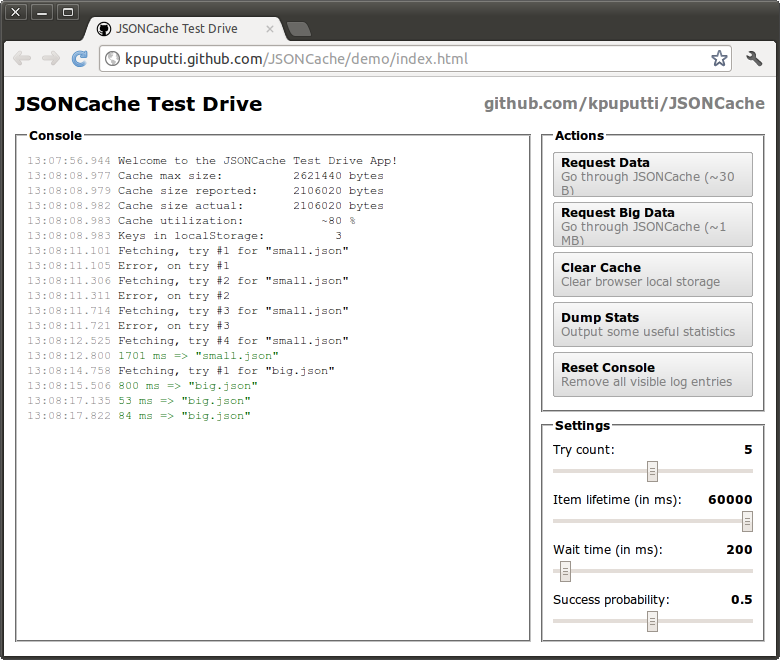
\includegraphics[width=\textwidth]{images/jsoncache-demo.png}
    \caption{Interactive JSONCache demo.}
    \label{figure:jsoncache-demo.png}
  \end{center}
\end{figure}
